\documentclass[financial_risks_lectures.tex]{subfiles}
\begin{document}

\subsection{Понятие Value at Risk (VaR)}
\setbeamercovered{transparent}
\begin{frame}{Понятие \textit{Value at Risk (VaR)}}
\begin{itemize}[<+->]
\item
\textit{Value at Risk (VaR)}  (стоимость портфеля, которой рискует инвестор) – это показатель риска инвестиций, который оценивает, какую часть стоимости могут потерять определенные инвестиции, при текущих рыночных условиях, за определенный промежуток времени. Наиболее распространенный период, для которого рассчитывается \textit{VaR}, - это один день или точнее – 24 часа. 
\item
\textit{VaR} обычно используется компаниями и регулирующими органами из финансового сектора экономики для оценки размера собственных средств организации, необходимых для покрытия возможных потерь.

\end{itemize}
\end{frame}

\begin{frame}{\textit{VaR }в теории финансовой математики и риск менеджмента}
\begin{itemize}[<+->]
\item
\textit{p VaR}, для данного портфеля, временного горизонта и доверительной вероятности \textit{p},  – это пороговая сумма потерь, такая что вероятность того, что убытки портфеля за данный период времени окажутся больше этой величины равна \textit{p}. 
\item
Допущения:
\begin{itemize}[<+->]
\item
При расчете \textit{VaR} для некоторого  временного интервала предполагается, что состав портфеля за этот период остается неизменным;
\item
пересчет стоимости портфеля происходит по текущим рыночным ценам (взятым с биржи).
\end{itemize}
\end{itemize}
\end{frame}

\begin{frame}
\begin{exampleblock}{Пример}
Если портфель акций имеет однодневный 5\% \textit{VaR }в размере 1 млн. руб., то это означает, что существует 5\% вероятность того, что этот портфель потеряет в стоимости более 1 млн. руб. в течение однодневного периода, если его состав не будет меняться. Иными словами, ожидается, что портфель принесет убытки в размере 1 млн. руб. или более хотя бы в один день из 20 (вследствие 5\% вероятности). \end{exampleblock}

Убыток, который оказался больше порогового значения называют пробоем \textit{VaR}.

\end{frame}
\subsection{Применение VaR}
\begin{frame}{Применение \textit{VaR}в финансах}

\begin{itemize}[<+->]
\item
риск менеджмент, 
\item
финансовый контроль, 
\item
финансовая отчетность,
\item
расчет регулирующими органами минимального размера капитала для финансовых организаций.
\end{itemize}
\end{frame}

\begin{frame}{}
\begin{block}{Минимальный размер собственных средств или достаточность собственного капитала}
\quad - это сумма капитала, которой должен обладать банк или другое финансовое учреждение, согласно требованиям регулирующего органа (например, центрального банка). 

\end{block}
\end{frame}

\begin{frame}[allowframebreaks]{Достаточность собственного капитала}
\begin{itemize}%[<+->]
\item
Показатель обычно выражен в виде коэффициента достаточности капитала, который определяется как доля собственных средств в активах, взвешенных с учетом риска.
\item
Данные ограничения устанавливаются государством для того, чтобы финансовые организации не имели сверхвысокого объема долга и не обанкротились. 
\pagebreak
\item
Требования по капиталу позволяют регулировать соотношение между собственными и заемными средствами организации (пассивная сторона баланса). Их не следует путать с резервными требованиями по депозитам, а также резервами ликвидности (минимально необходимая доля активов, хранимая в виде наличности и высоколиквидных активов).
\end{itemize}
\end{frame}

\begin{frame}[shrink=10]{Другие области применения \textit{VaR}}
 \begin{itemize}[<+->]
 \item 
\textit{VaR }используется доверительными управляющими инвестиционных фондов, пенсионных фондов, фондов пожертвований. Управляющие могут применять показатели VaR как к фонду в целом, таки и к отдельным его частям, управляемым по индивидуальной стратегии.  
\item
Вместо вероятности потерь обычно определяется максимальная сумма допустимых потерь по каждому направлению. Это обеспечивает простые средства контроля и ограничения потерь в рамках определенного риска. 
\item
\textit{VaR }как ожидаемая сумма потерь, более доступен для понимания, нежели стандартное отклонение доходности активов.

 \end{itemize}
\end{frame}
\subsection{Формула VaR}
\begin{frame}[shrink=10]{Математическое определение \textit{VaR}}

Для заданного уровня доверительной вероятности $\alpha\in (0;1)$, \textit{VaR} портфеля - это наименьшее число \textit{l}, такое что вероятность того, что убытки \textit{L} превысят \textit{l} составлет не больше чем $(1-\alpha)$.
В терминах математики, если \textit{L} это убыток портфеля, то $\operatorname{VaR}_{\alpha}(L)$ это квантиль уровня $\alpha$, т.е.
\begin{align}
\operatorname{VaR}_\alpha(L) & \nonumber
=\inf\{l \in \mathbb{R}:P(L>l)\le 1-\alpha\}\\ &
=\inf\{l\in \mathbb{R}:F_L(l) \ge \alpha\}\end{align}
$\inf$ - нижняя граница множества. Если минимальный элемент множества существует, то его нижняя граница совпадает с минимумом.\\
Формула предполагает, что известна функция распределения вероятностей убытков, поэтому данный подход может быть использован только для параметрической \textit{VaR}.
\end{frame}
\begin{frame}
\begin{block}{Определение}
Квантилью уровня $\alpha$ , или $\alpha$-квантилью, $(0<\alpha<1)$ случайной величины \textit{X} (распределения случайной величины \textit{X}) называют такое значение $x_{\alpha}$ этой случайной величины, меньше которого \textit{X} принимает значение с вероятностью $\alpha$, т.е. $F(x_{\alpha}) = P(x < x_{\alpha}) = \alpha$. 
\end{block}
\end{frame}


\begin{frame}{Методики определения VaR}
\begin{itemize}
\item
параметрические (аналитические или дисперсионно-ковариационные);
\item
непараметрические модели. 
\end{itemize}
Модель называется параметрической, если известна функция распределения случайной величины и параметры ее распределения.

Предположения: доходность финансовых активов следует определенному виду вероятностного распределения, обычно нормального. 

\end{frame}
\begin{frame}[shrink=10]{Параметрический \textit{VaR}}
Используя прошлые данные статистики, определяют ожидаемые значения доходностей, дисперсий и ковариаций доходностей активов. 

На их основе рассчитывают \textit{VaR }портфеля для заданного уровня доверительной вероятности по формуле:
\begin{align}
VAR_p=P_p \sigma_p z_{\gamma},
\end{align}
где
- \textit{VaR }порфеля;

$P_p$ - стоимость портфеля;

$\sigma_p$ - стандартное отклонение доходности портфеля, соответствующее времени, для которого рассчитывается~\textit{VaR};

$z_{\gamma}$ - количество стандартных отклонений, соответствующих уровню доверительной вероятности~$\gamma$.

\end{frame}
\begin{frame}{Абсолютный и относительных \textit{VaR}}
Абсолютный \textit{VaR }– это максимальная сумма денег, которую может потерять портфель инвестора в течение определенного времени с заданной доверительной вероятностью. 

Относительный \textit{VaR }отличается от абсолютного тем, что он рассчитывается относительно ожидаемой доходности потфеля.
\end{frame}
\setbeamercovered{invisible}
\begin{frame}{Определение однодневного \textit{VaR} I}
\begin{exampleblock}{Пример}
Определить однодневный \textit{VaR }с доверительной вероятностью 90\% для портфеля стоимостью 10~млн.~руб., в который входят акции только одной компании. Стандартное отклонение доходности акции в расчете на день равно 1.5\%.
Решение:
\begin{align*}
VaR &=10 \text{ млн. руб.}\times 1.5\% \times \onslide<2-> {1.28} \\ 
&=\onslide<3->{0.192 \text{ млн. руб}}\end{align*}
\end{exampleblock}
\end{frame}
\setbeamercovered{transparent}
\begin{frame}{Определение Z-значения}
% Table generated by Excel2LaTeX from sheet 'Лист1'
\begin{table}[htbp]
  \centering
  \caption{Наиболее часто используемые значения функции стандартного нормального распределения}
  \begin{tabular}{rl}
    \begin{tabular}{cc}
    \toprule
    \textbf{$z_{\gamma}$-значение} & $\gamma$ \\
    \midrule
    1,280  & 0,900 \\
    1,645 & 0,950 \\
    1,960  & 0,975 \\
    2,575 & 0,995 \\
    \bottomrule
    \end{tabular}%
	&
	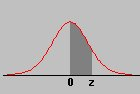
\includegraphics[scale=0.6]{img/normal_distribution.png}  
  \end{tabular}
  \label{tab:addlabel}%
\end{table}%

$z_{\gamma}$ - количество стандартных отклонений, соответствуюищих доверительной вероятности $\gamma$;

$\gamma$ - доверительная вероятность, площадь под графиком нормальной кривой.

\end{frame}
\subsection{Параметрическая модель VaR}
\begin{frame}[shrink=10]{Оценка ошибки параметрической модели \textit{VaR}} 
VaR портфеля рассчитывается на основе выборочных данных за определенный период времени. В результате возникает необходимость оценить доверительный интервал для полученного значения \textit{VaR}. 
Мы предполагаем, что доходность портфеля имеет нормальное распределение. Наилучшей оценкой дисперсии нормального распределения является "исправленная" дисперсия:
\begin{align}
s^2=\frac{1}{n-1}\sum\limits_{i=1}^n(X_i-\overline{X})^2,
\end{align}
где $s^2$ - "исправленная" дисперсия;

$X_i$ - значение случайной величины для \textit{i}-ой выборки; 

$\overline{X}$ - среднее значение случайной величины; 

\textit{n} - количество выборочных данных.

\end{frame}
\begin{frame}[shrink=10]
\begin{align*}
\frac{s^2}{\sigma^2} & =\frac{1}{n-1}\sum_{i=1}^n\left(\frac{X_i-\overline{X}}{\sigma}\right)^2
\end{align*}
Величина $\sum\limits_{i=1}^n\left(\frac{X_i-\overline{X}}{\sigma}\right)^2$ имеет распределение хи-квадрат $\chi^2$ с $n-1$ степенями свободы. 
\begin{align}
\frac{(n-1)s^2}{\sigma^2} & =\sum_{i=1}^n\left(\frac{X_i-\overline{X}}{\sigma}\right)^2
\end{align}
Необходимо найти границы интервала, который бы с доверительной вероятностью $\gamma$ накрывал истинное значение дисперсии случайной величины:
\begin{align}
P(\chi_1^2<\chi^2<\chi_2^2)=\gamma
\end{align}
\end{frame}
\begin{frame}
Значения конечных точек доверительного интервала обычно выбирают таким образом, чтобы вероятности событий $\chi^2<\chi_1^2$ и $\chi^2>\chi_2^2$ были одинаковыми. Пусть эта вероятность равна $\alpha$, тогда
\begin{align}
P\left[\chi_{\alpha}^2<\frac{(n-1)s^2}{\sigma^2}<\chi_{1-\alpha}^2\right] & =1-2\alpha \nonumber \\
P\left[\frac{\chi_{\alpha}^2}{(n-1)s^2}<\frac{1}{\sigma^2}<\frac{\chi_{1-\alpha}^2}{(n-1)s^2}\right] & =1-2\alpha \nonumber \\
P\left[\frac{(n-1)s^2}{\chi_{1-\alpha}^2}<\sigma^2<\frac{(n-1)s^2}{\chi_{\alpha}^2}\right] & =1-2\alpha
\end{align}
\end{frame}

\begin{frame}{Границы доверительного интервала дисперсии}
По таблице квантилей распределения $\chi^2$ находим нижнюю и верхнюю границы доверительного интервала дисперсии случайной величины. Квадратные корни из данных значений представляют собой нижнюю $\sigma_L$  и верхнюю $\sigma_U$ границы доверительного интервала стандартного отклонения.

Если в качестве случайной величины выступает доходность портфеля, то найденные значения сигм показывают доверительные границы стандартного отклонения доходности портфеля.

Т.о., доверительный интервал для \textit{VaR} портфеля определяется по формулам:
\begin{align}
VaR_L &=P_p \cdot \sigma_L \cdot z_{\gamma},\\
VaR_U &=P_p \cdot \sigma_U \cdot z_{\gamma},
\end{align}

\end{frame}

\setbeamercovered{invisible}
\begin{frame}
\begin{exampleblock}{Пример}
Однодневный \textit{VaR }портфеля из двух акций составляет 267.3 тыс. руб. Дисперсия доходности портфеля равна 2.628, стандртное отклонение, соответственно, 1.62\%. Данный результат был получен на основе данных по доходности акций за 101 день. Требуется определить доверительный интервал для \textit{VaR }с коэффициентом доверия $\gamma = 0,95$.
\end{exampleblock}
\end{frame}
\begin{frame}[shrink=10]
\begin{exampleblock}{Решение}
Из соотношения $\gamma=1-2\alpha$ находим значение $\alpha$, соответствующее доверительной вероятности 95\%:
\onslide<2->{$$\alpha=\frac{1-0.95}{2}=0.025$$}

\end{exampleblock}
\end{frame}

\begin{frame}[shrink=15]
\begin{table}[htbp]
  \centering
  \caption{Критические области для хи-квадрат распределения}
\begin{tabular}{rl}
% Table generated by Excel2LaTeX from sheet 'Лист1'
    \begin{tabular}{rrrrr}
    \toprule
    \textbf{p/df} & \textbf{25} & \textbf{50} & \textbf{75} & \textbf{100} \\
    \midrule
    \textbf{0.95} & 37,65248 & 67,50481 & 96,21667 & 124,3421 \\
    \textbf{0.975} & 40,64647 & 71,4202 & 100,8393 & 129,5612 \\
    \textbf{0.05} & 14,61141 & 34,76425 & 56,05407 & 77,92947 \\
    \textbf{0.025} & 13,11972 & 32,35736 & 52,94194 & 74,22193 \\
    \bottomrule
    \textbf{p/df} & \textbf{125} & \textbf{150} & \textbf{175} & \textbf{200} \\
    \bottomrule
    \textbf{0.95} & 152,0939 & 179,5806 & 206,8668 & 233,9943 \\
    \textbf{0.975} & 157,8385 & 185,8004 & 213,5236 & 241,0579 \\
    \textbf{0.05} & 100,1782 & 122,6918 & 145,4058 & 168,2786 \\
    \textbf{0.025} & 95,94573 & 117,9845 & 140,2619 & 162,728 \\
    \bottomrule
    \textbf{p/df} & \textbf{225} & \textbf{250} & \textbf{275} & \textbf{300} \\
    \bottomrule
    \textbf{0.95} & 260,9921 & 287,8815 & 314,6784 & 341,3951 \\
    \textbf{0.975} & 268,4378 & 295,6886 & 322,8293 & 349,8745 \\
    \textbf{0.05} & 191,2808 & 214,3916 & 237,5948 & 260,8781 \\
    \textbf{0.025} & 185,3483 & 208,0978 & 230,9574 & 253,9123 \\
    \bottomrule
    \end{tabular}%
&
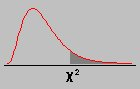
\includegraphics[scale=0.6]{img/chi2area.png}\\
\end{tabular}
  \label{tab:addlabel}%
\end{table}
\end{frame}

\begin{frame}[shrink=15]
\begin{exampleblock}{Решение}
По таблице квантилей распределения $\chi^2$ находим квантили $\chi_{1-\alpha}^2$ и $\chi_{\alpha}^2$ со степенями свободы 100, и определяем границы доверительного интервала для дисперсии.
\begin{align*}
\frac{(n-1)s^2}{\chi_{0.975}^2} &=\onslide<2->{\frac{100 \cdot 2.628}{129.56}=}\onslide<3->{2.06854}\\
\sigma_L&=\onslide<4->{1.44\%}\\
\frac{(n-1)s^2}{\chi_{0.025}^2}&=\onslide<5->{\frac{100 \cdot 2.628}{74.22}=}\onslide<6->{3.54083}\\
\sigma_U&=\onslide<7->{1.88\%}\\
VaR_L&=\onslide<8->{237,6}\\
VaR_U&=\onslide<9->{310,2}
\end{align*}
Таким образом, с доверительной вероятностью 95\% процентов можно быть уверенным, что действительное значение \textit{VaR} лежит в границах от 237,6 тыс. руб. до 310,2 тыс. руб.

\end{exampleblock}
\end{frame}
\setbeamercovered{transparent}
\subsection{Средние ожидаемые потери}
\begin{frame}{Средние ожидаемые потери}{Conditional Value at Risk (CVaR), Average Value at Risk (AVaR), expected tail loss (ETL)}
\begin{block}{\textbf{Средние ожидаемые потери (Expected shortfall, ES)}}
- это способ измерения и одновременно показатель финансового риска портфеля инвестиций или кредитов. Ожидаемые потери на $\gamma\%$ уровне – это ожидаемая доходность портфеля в худших $\gamma\%$ случаев. Средние ожидаемые потери являются предпочтительной альтернативой \textit{VaR}, поскольку показатель более чувствителен к форме графика плотности распределения вероятностей в его хвостовой части.
\end{block}
\end{frame}

\begin{frame}[shrink=15]
Ожидаемая доходность \textit{X }и \textit{Y} составляет, соответственно 3\% и 1\% (см. рис. \autoref{fig:df}).

Стандартные отклонения доходностей \textit{X} и \textit{Y} равны 10\%.
\begin{figure}
	\centering
	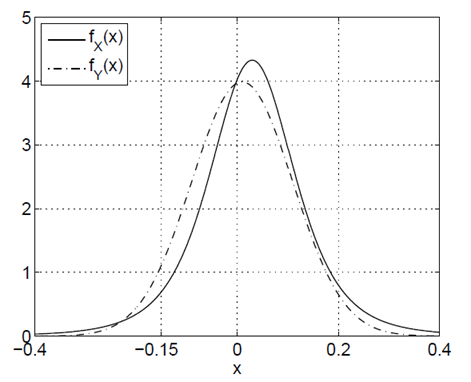
\includegraphics[scale=0.6]{img/expected_shortfall_df.png}
	\caption{Графики функций плотности распределения доходностей финансовых инструментов \textit{X }и \textit{Y}}
	\label{fig:df}	
\end{figure}
\end{frame}

\begin{frame}[shrink=25]
Графики функций $F_X(x), F_Y(x)$ пересекаются в точке $x=-0.15$, $F_X(-0.15)=F_Y(-0.15) = 0.05$ (см. рис. \ref{fig:cdfs}). 
\begin{figure}
	\centering
	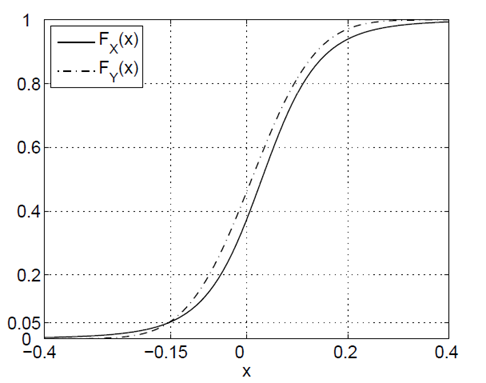
\includegraphics[scale=0.6]{img/expected_shortfall_cdfs.png}
	\caption{Графики кумулятивных функций распределения доходностей финансовых инструментов \textit{X }и \textit{Y}}\label{fig:cdfs}
\end{figure}
Оба финансовых инструмента могут потерять более чем 15\% их текущей стоимости с вероятностью 5\%. 

Мы можем заключить, что они одинаково рискованные, потому что их 95\% \textit{VaR} одинаковые.  
\end{frame}

\begin{frame}{Недостаток \textit{VaR }}
Если бы мы обосновывали выбор финансовых инструментов соотношением стандартного отклонения их доходности и ожидаемой доходности, то мы могли бы заключить, что поскольку стандартные отклонения одинаковые, то инструмент \textit{X} более предпочтителен, потому что имеет более высокую ожидаемую доходность. 

\textbf{На самом деле верен противоположный вывод.}

В обоих случаях \textit{VaR }равен 0.15, однако \textit{X }имеет более толстый хвост и, следовательно, более рискованный. Недостатком \textit{VaR }является то, что показатель не дает никакой информации о размерах потерь за пределами порогового уровня.

\end{frame}
\begin{frame}[allowframebreaks]{Преимущества показателя средних ожидаемых потерь}
\begin{figure}	
	\centering
	\begin{subfigure}[t]{4.1cm}
		\centering
		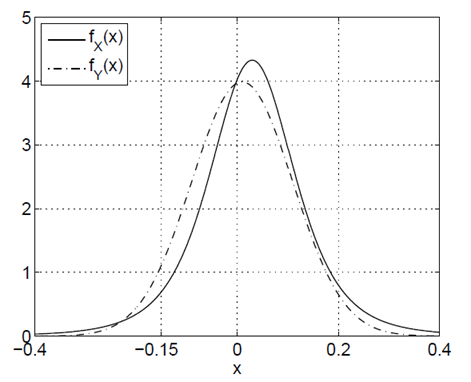
\includegraphics[scale=0.3]{img/expected_shortfall_df.png}
	\caption{Функция плотности распределения}\label{fig:a_df}	
	\end{subfigure}
	\quad
	\begin{subfigure}[t]{4.1cm}
		\centering
		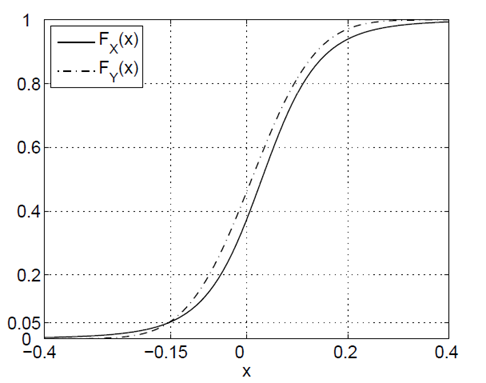
\includegraphics[scale=0.3]{img/expected_shortfall_cdfs.png}
		\caption{Кумулятивная функция распределения}\label{fig:b_cdf}
	\end{subfigure}
	\caption{Графики функций распределения доходностей финансовых инструментов \textit{X }и \textit{Y}}\label{fig:df_and_cdf}
\end{figure}
Показатель средних ожидаемых потерь оценивает риск инвестиций консервативным способом, фокусируясь на менее прибыльных исходах. 

\pagebreak

Для больших значений доверительной вероятности $\gamma$, показатель игнорирует более прибыльные, но маловероятные варианты, в то время как для малых значений доверительной вероятности $\gamma$, он фокусируется на самых больших потерях. 

С другой стороны, вопреки подходу дисконтирования максимального убытка, даже для малых значений доверительной вероятности $\gamma$ показатель средних ожидаемых потерь принимает во внимание не только одиночный наиболее катастрофичный вариант. 
На практике значение доверительной вероятности $\gamma$ выбирается равным 5\%.

\end{frame}
\subsection{Формула CVaR}
\begin{frame}{Средние ожидаемые потери}{Формальное определение}
Если \textit{X }это поступления от портфеля за некоторый будущий период времени и $\alpha$ - это число $0<\alpha<1$, тогда сумма ожидаемых потерь определяется по формуле:
\begin{align}
\label{es}
ES_{\alpha} = \frac{1}{\alpha}\int_0^{\alpha} \mbox{VaR}_{\gamma}(X)d\gamma,
\end{align}
где  $\mbox{VaR}_{\gamma}$ - это \textit{VaR} с доверительной вероятностью $\gamma$.

Таким образом, это средний ожидаемый (математическое ожидание) размер убытка в денежных единицах (с данным уровнем риска, на данном временном горизонте), при условии, что он превысит значение $VaR_{\gamma}$.
\end{frame}

\begin{frame}
Если мы предполагаем, что доходность портфеля имеет нормальное распределение со средним значением равным нулю и стандартным отклонением $\sigma$, тогда величина средних ожидаемых потерь вычисляется по формуле:
\begin{align}
\label{es_normal}
ES=\frac{\sigma}{(\gamma-1)\sqrt{2\pi}}e^{-\frac{VaR_{\gamma}^2}{2\sigma^2}}
\end{align}

\end{frame}
\setbeamercovered{invisible}
\begin{frame}
\begin{exampleblock}{Пример}
Определите величину средних ожидаемых потерь для одного дня для портфеля стоимостью 5 млн. руб., в который входят акции только одной компании. Стандартное отклонение доходности акции в расчете на день равно 2,5\%. Предполагается, что доходность акции имеет нормальное распределение. Доверительная вероятность равна 90\%.
\end{exampleblock}
\end{frame}
\begin{frame}
\begin{exampleblock}{Решение}
VaR портфеля для уровня доверительной вероятности 90\% равен:

\onslide<2->
$VaR_{0,9}=5\cdot 0,025\cdot 1,28=160 \text{ тыс.руб.}$

\onslide<3->
Стандартное отклонение дохода портфеля: 

\onslide<4->
125~тыс.~руб.

\onslide<5->
Согласно формуле, величина средних ожидаемых потерь для одного дня для доверительной вероятности 90\% составляет: 

\onslide<6->
220~тыс.~руб.
\end{exampleblock}
\end{frame}
\setbeamercovered{transparent}
\end{document}
